\documentclass[conference]{IEEEtran}

\usepackage{graphicx}
\usepackage{amsmath}
\usepackage{algorithmic}
\usepackage{array}
\usepackage{url}
\usepackage{listings}
\usepackage{tabu}


\begin{document}

\title{Rapid-Rate: A Framework for Semi-supervised \\Real-time Sentiment Trend Detection\\ in Unstructured Big Data}

\author{
    \IEEEauthorblockN{Vineet John}
    \IEEEauthorblockA{
        David R. Cheriton School of Computer Science\\
        University of Waterloo\\
        Waterloo, Ontario N2L 3G1\\
        Email: vineet.john@uwaterloo.ca
    }
}

\maketitle

\begin{abstract}
    Commercial establishments (like restaurants, service centers) have several sources of feedback, most of which need not be as structured as feedback provided by services like Yelp, or Amazon.
    Services like these provide a fine-grained score for product and service ratings.
    Some sources, however, like social media (Twitter, Facebook), mailing lists (Google Groups), forums (Quora) et al. are sources for much more volumnious, but unstructured and unlabeled data. 
    This text could be pipelined into a system with a built-in prediction model, with the objective of generating real-time graphs on opinion and sentiment trends. 
    Although such tasks like the one described about have been explored with respect to document classification problems in the past, the implementation described in this paper, by virtue of learning a continuous function rather than a discrete one, offers a lot more depth of insight as compared to document classification approaches. 
    This study aims to explore the validity of such a continuous function predicting model to quantify sentiment about an entity, without the additional overhead of labeling, pre-processing, and feature extraction.
\end{abstract}

\providecommand{\keywords}[1]{\textbf{\textit{Keywords---}} #1}
\keywords{natural language processing, big data, word embedding, regression, time-series analytics}

\IEEEpeerreviewmaketitle

\vspace{5mm}

\section{Introduction}
    Document labeling and attribute discovery is already a widely researched area in the domain of natural language processing.
    The most common use-cases of document classification are product \& service review rating predictions, automatic grading of essays, spam detection, plagiarism detection et al.
    However, most of the current approaches used for these tasks rely on lexicon based methods with a centralized source indicating the weights of a word towards a set of emotion or sentiment.
    Some other approaches use N-gram count vectorization approaches and document level similarity scores like TF-IDF.
    However, N-gram approaches only partially model the language context probabilities i.e. the probably of a word occurring next in the corpus depends only on the n-1 words that precede it.
    Word2Vec's model take additional word contexts into account, a feature which will be elaborated upon later in this paper Section \ref{Word2Vec}.

    However, models like these are difficult to train for the following reasons:
    \begin{itemize}
      \item Having to hand-pick features
      \item Having to manually re-train the models on subset of the features to determine the best-fit
      \item Having to use stepwise regression to eliminate non-relevant features
    \end{itemize}

    All of the processes described above are time-consuming and tedious. 
    The objective of this work is to implement and evaluate a strategy to effectively eliminate the above steps from the process of training a language model. 
    The proposition is to rely on unsupervised strategies like continuous bag-of-words and the skip-gram model to learn word embeddings, that will serve as a syntactic and semantic proxy for the text being processed. 
    The features thus learnt, can then be used to train regression models to predict text scores.

\begin{figure*}[ht] \label{fig:word2vec-vectorspace-intuition}
    \centering
    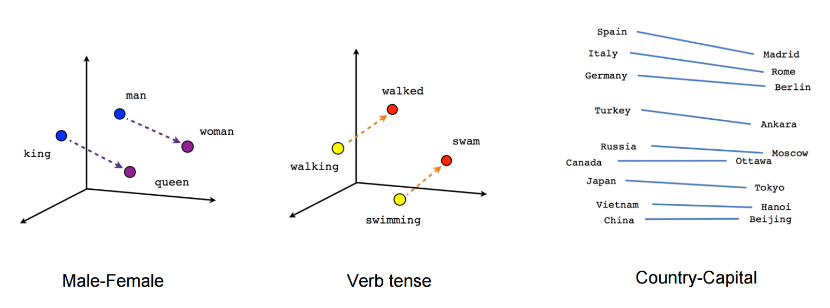
\includegraphics[width=\textwidth]{images/word2vec_1.png}
    \caption{Word2Vec Vector Space Intuition\cite{tensorflow_word2vec}}
\end{figure*}

\vspace{5mm}

\section{Similar Work}
    This section discusses the previous work done on mining and analytics pertaining to text data.

    Most of the similar work in the area of learning word-embeddings is related to classifying documents into a given set of labels or topics. 
    The purpose of this study is to extend the usage of the document vector representation to demonstrating its usage when the response variable (the output of a learning task) a continuous function (document-scoring) rather than discrete values (document classification). This work can be viewed as a generalization of the previous approaches, because this study aims to predict fine-grained document scores, rather than coarse document classifications.

    Most of the current work in usage of regression techniques on text content are related to metadata or features extraction \cite{su2015genetic} \cite{weissman2016natural}. Similarly there have been several studies to identify document tags using classification techniques\cite{bespalov2011sentiment}\cite{pang2002thumbs}. However, there is a relative absence of studies to evaluate the accuracy of regression models that try to predict a document score using a continuous-function model.

    As far the the author is aware, there has been no similar work to test the regression accuracy of paragraph vectors in an experimental research setup before. Hence, the evaluation of the effectiveness of this approach will be assessed using a generic evaluation metric.

\vspace{5mm}

\section{Problem Statement} \label{problem_statment}
    The problem statement can be formulated as an evaluation of Paragraph Vectors\cite{le2014distributed} on a document score regression task to evaluate the accuracy of the prediction model that can be built using the shallow neural network language model learning algorithm previously descibed by Mikolov et al. \cite{mikolov2013efficient}, which was primarily used to unsupervisedly train word embeddings.

    The prediction scores will be evaluated using the co-efficient of determination metric, also known as the R\textsuperscript{2} metric \cite{cameron1997r}. The hypothesis is to prove that the document ratings have a positive correlation with the vectorized versions of the document text content, because the semantics of positive and negative reviews are expected to be captured by the shallow neural network trained on the corpus. The expected R\textsuperscript{2} metric score being over 0, will confirm the hypothesis, and a negative value will contradict it.

\begin{figure*}[ht] \label{fig:paragraph-vector-framework}
    \centering
    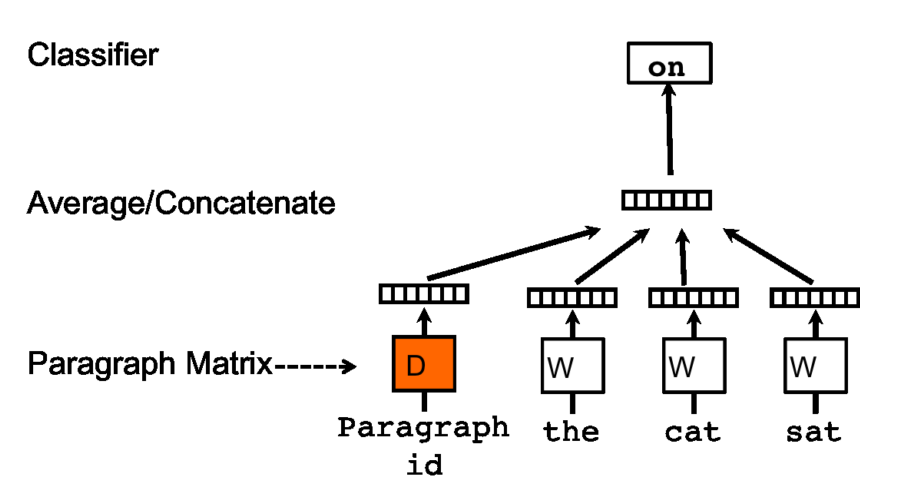
\includegraphics[width=400pt]{images/docvec_1.png}
    \caption{Paragraph Vector Learning Framework\cite{mikolov2013distributed}}
\end{figure*}

\vspace{5mm}

\section{Motivation}
    The motivation for the project is to prove that a substantial amount of the semantic signal about sentiment with respect to a product or service, as extracted from a snippet or document of text, should prove to be a good indicator of the labeled document scores. If proven to be true, the objective includes building a real-time streaming framework, which can analyze unseen reviews from the previously provided exampled of unlabeled data, and be able to emit a score-prediction with minimal processing delays. This framework can be set-up on commodity hardware, and a given business can simply pipe their unlabeled reviews or articles into the system, and expect a graphical representation of the sentiment about a particular topic that is updated in real-time. The framework also allows rules to be set for alerts, so, for instance, if the approval rating of a particular business falls very low, an email alert could be triggered to the business decision makers to respond quicker to the negative sentiment, a process which would otherwise span several business days.

    \subsection{Semi-supervised Learning}
        The statistical learning formulation of the problem statement in this study, can be broken down into two distinct segments, namely:
        \begin{itemize}
            \item Learning a projection of the document into vector space. This projection will act as a mathematical proxy for the sentiment that the document is trying to convey. This segment is completely unsupervised, and does not require any tuning or pre-processing to compute.
            \item Learning a relation between the aforementioned projection of each labeled document, and the associated score or label. This segment of the learning pipeline is supervised relies on previously scored or rated documents.
        \end{itemize}

    \subsection{Continuous function learning}
        Assume that a given output variable \textit{y} depends on a variable \textit{x} such that
        \begin{equation}
            \displaystyle f(x) = \beta x + c + \epsilon
        \end{equation}

        \begin{equation}
            \displaystyle y = f(x)
        \end{equation}
        where x represents a vector of independent variables, y represents the dependant or response variable, $\beta$ and c are model vector space functions that are applied to x to map it to y, and $\epsilon$ is the error term.

        Now, assume that the variable \textit{x} increases by a small amount $\Delta x$, and that $x_0$ was the initial value, such that the value of \textit{x} is updated to
        \begin{equation}
        \displaystyle \Delta x = x - x_0
        \end{equation}

        A continuous function is defined as one in which an infinitely small change for the input variable x results in a corresponding infinitely small change in the response variable y \cite{continuous_function}, which can be expressed as
        \begin{equation}
        \displaystyle \Delta y = f(x) - f(x_0)
        \end{equation}

        Continuous functions are typically needed when the response variable calculated is a measurable quantity, rather than a class label. Since sentiment as fine-grained values offer more depth in terms of sentiment insight \cite{drake2008sentiment}, the study in this paper is formulated as a regression problem.

\vspace{5mm}

\section{Challenges}

    \subsection{Language Model Learning}
        

    \subsection{Unstructured Big Data}

    \subsection{Deep Learning}

\vspace{5mm}

\begin{figure*}[ht] \label{fig:system-architecture}
    \centering
    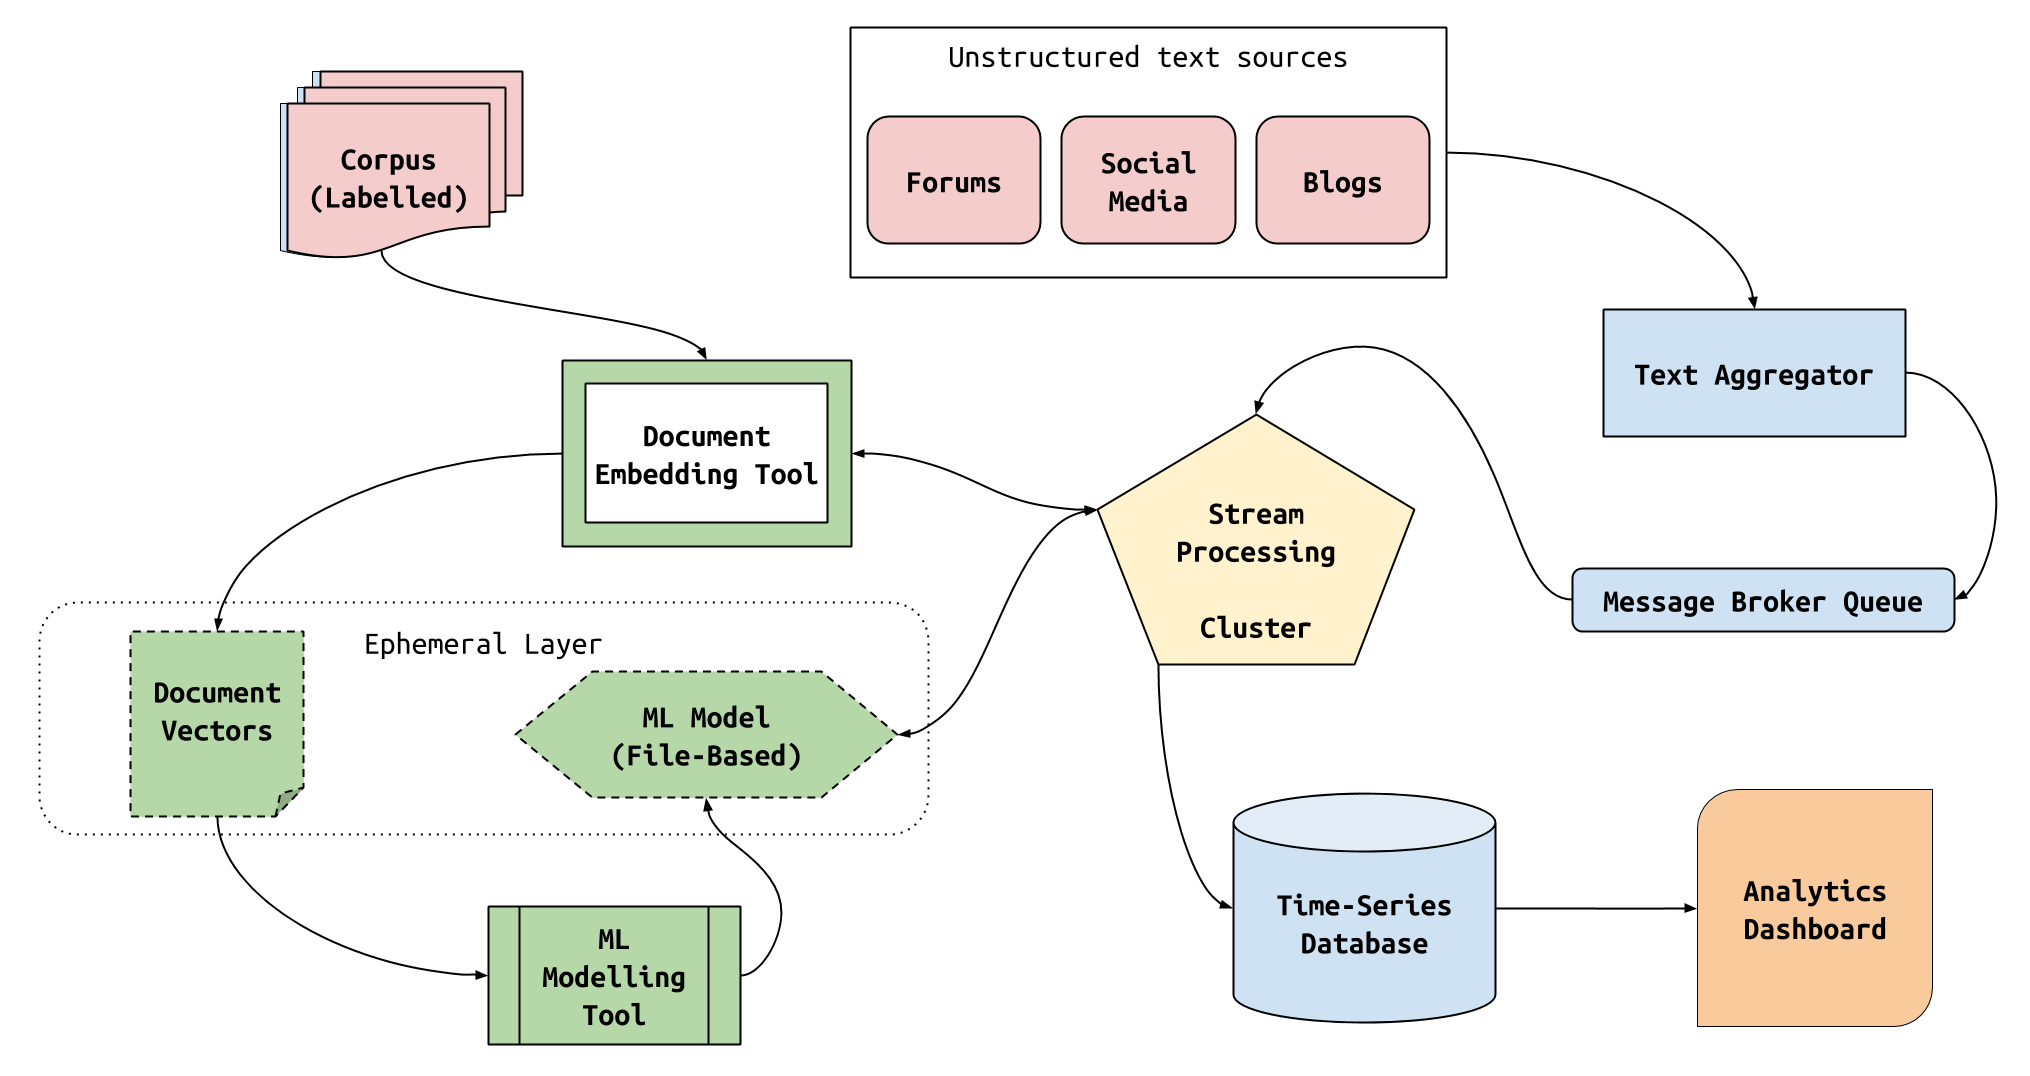
\includegraphics[width=\textwidth]{images/rapid_rate_system_arch_1.png}
    \caption{Rapid-Rate System Architecture}
\end{figure*}

\section{Background}

    \subsection{Word2Vec} \label{Word2Vec}
        Word vectors are a step-away from the traditional bag-of-words + n-gram model. The latter ends up losing

        The Word2Vec model\cite{mikolov2013efficient} can take into consideration both preceding and succeeding words, to compute the probabililty of occurrence of the current word, as part of the Continuous Bag-of-words (CBOW) model. Alternatively, Word2Vec also provides a skip-gram model\cite{mikolov2013distributed}, which conversely, used the context of a word i.e. the words preceding and following it, to predict the most statistically probably current word. These word embeddings can be used to derive both syntactic as well as symantic relations in the vector space of the language model. A representation of this is given in Figure \ref{fig:word2vec-vectorspace-intuition}.

    \subsection{Paragraph Vectors}
        Paragraph vectors are a similar concept to Word2Vec, but rely on computing a fixed-length vector representation of a variable length group of words, which could be a sentence, a paragraph, or even an entire document.

        Since vectors representations of documents seem to outperform bag-of-words models for the purposes of semantic summarization and document classification tasks, it follows that a vector representation based approach should be used to evaluate performance on a regression task as well. Paragraph vectors also address some of the keyweaknesses of bag-of-words models. First, they inherit an important property of theword vectors: the semantics of the words. The second advantage of the paragraph vectors is that they take into consideration the word order, at least in a small context, in the same way that an n-grammodelwith a large n would do. This is important, because the n-gram model preserves a lot of information of the paragraph, including the word order\cite{le2014distributed}. The paragraph representation framework is depicted in Fig. \ref{fig:paragraph-vector-framework}.

        The implementation of paragraph vectors used for the purpose of implementing the system architecture in this study is Doc2Vec, from the Gensim library\cite{doc2vec_api}.


    \subsection{Statistical Learning Models}
        Once the entities about which we wish to learn a representation are projected into vector space, there are an abundance of statistical learning methods that can be used to learn a continuous function including linear regression, polynomial regression, ridge regression, stepwise regression, lasso regression et. al.

        This study utilizes linear regression and support vector regression to test the veracity of the model predictions. Both these methods are described in the below subsections.

    \subsubsection{Linear Regression}
        The problem of regression in mathematical statistics is characterized by the fact that there is insufficient information about the distributions of the variables under consideration\cite{regression_analysis}.

        In the case for this study, once the Doc2Vec implementation generates the vector space representation of each of the documents, each of the learned dimensions reprsent a different input variable for the regression problem. In reality, each of these dimensions represent a weighted probabilty score generate by the hidden layer of neurons in the paragraph vector model.

    \subsubsection{Support Vector Regression}
        Support Vector Regression (SVR) attempts to minimize the generalization error bound so as to achieve generalized performance. The idea of SVR is based on the computation of a linear regression function in a high dimensional feature space where the input data are mapped via a nonlinear function. SVR has been applied in various fields – time series and financial (noisy and risky) prediction, approximation of complex engineering analyses, convex quadratic programming and choices of loss functions\cite{basak2007support}.

        The input parameters to the support vector regressor remain the same as those described above for the linear regressor.


    \subsection{Distributed Messaging with Kafka}
        This project uses Apache Kafka for processing huge volume of real-time data streams. Like a messaging system, Kafka employs a pull-based consumption model that allows an application to consume data at its own rate and rewind the consumption whenever needed. By focusing on log processing applications, Kafka achieves much higher throughput than conventional messaging systems. It also provides integrated distributed support and can scale out. Kafka has been used successfully at LinkedIn for both offline and online applications. \cite{kreps2011kafka}

    \subsection{Horizontal Scaling with Spark Streaming}
        This study used Apache Spark Streaming for the real-time processing of the unlabeled document data. Discretized streams (D-Streams), a stream programming model for large clusters that provides consistency, efficient fault recovery, and powerful integration with batch systems is the core offering of Spark Streaming. The key idea is to treat streaming as a series of short batch jobs, and bring down the latency of these jobs as much as possible. This brings many of the benefits of batch processing models to stream processing, including clear consistency semantics and a new parallel recovery technique that is a truly cost-efficient recovery technique for stream processing in large clusters\cite{zaharia2012discretized}.

\vspace{5mm}

\section{System Architecture}
    The system architecture is depicted in Fig. \ref{fig:system-architecture}

    The individual components and their interactions are described in the below sub-sections \ref{Components} and \ref{Component Interactions}.

    \subsection{Components} \label{Components}

        \subsubsection{Document embedding tool}
            The labeled documents are the initial input parameters to the Rapid-Rate framework. These are variable length text snippets or paragraphs, each with an associated score. This tool is used to convert the document text into their corresponding vector representations.

        \subsubsection{ML Modeling tool}
            This is a library used by the framework to infer a model from the vectorized documents (independent variable) that predict the rating/score of that particular document (dependent variable). 

        \subsubsection{Text Aggregator}
            This component is responsible for merging multiple different streams of data into a unified stream that can be used to predict sentiment ratings of unlabeled documents.

        \subsubsection{Message Broker Queue}
            This component acts as the arbiter for the incoming unlabeled documents. 
            Each document is read from the queue and is processed in turn.

        \subsubsection{Stream Processor}
            The stream processor is responsible for reading and processing the unlabeled documents, predicting the score/rating of each incoming document, and forwarding the scores for further usage.

        \subsubsection{Time-Series Database}
            A time series database is optimized to handled collections of data objects that are indexed by time. 
            It supports fast querying of data over temporal scan ranges and is ideal for time-series based analytics

        \subsubsection{Analytics Dashboard}
            The analytics dashboard provides a visual representation of overall sentiment over time, and supports setting alerts to warn the end-user when overall sentiment dips below a certain user-defined threshold.

    \subsection{Component Interactions} \label{Component Interactions}
        A simple processor reads the labeled documents and feeds it into the Document embedding tool, which, in turn, emits a representation of each of the labeled documents as a vector.
        The vectors representations of the documents are now associated with their corresponding scores and the vector representations and the scores fed together into the ML Modeling tool to generate Linear Regression and Support Vector Regression models. 
        These models are then `pickled' or flushed to disk, to be used by the real-time prediction module. 
        Along with these models, the trained Document embedding model is also flushed to disk.

        Once these models are flushed to disk, the system can kickstart it's real-time prediction framework. 
        The unlabeled documents are published to the message broker queue, to which the daemon component of the architecture is subcribed to. 
        It processes lists of documents in micro-batches and emits a list of scores. 
        These scores are posted in real-time to a time-series database, which in turn, acts as the data backend for the analytical dashboard.

        The analytical dashboard provides a line graph of the sentiment trend over time, and can also provided for additional features such as Bollinger Band plotting, and threshold-breach based alerts.

\vspace{5mm}

\section{Implementation}

    The primary language of implementation of this research project is Python, and the other frameworks and components have been described in the Tech Stack section. (Section \ref{Tech stack})

    \subsection{Offline learning model}


    \subsection{Online real-time prediction engine}


    \subsection{Tech stack} \label{Tech stack}
        The tech stack used for the implementation of the framework is comprised of:

        \subsubsection{Python}
            Processing code, pipelining, real-time prediction code\cite{python}.

        \subsubsection{Gensim}
            Python library. The Doc2Vec class in Gensim is used to learn the document representations\cite{doc2vec_api}.
        
        \subsubsection{Scikit-Learn}
            Python libary. The linear regression and support vector regression is done using this library\cite{scikit_learn}.
        
        \subsubsection{Apache Kafka}
            Distributed messaging queue. This is used to receive new unlabeled documents, and is also a potential sink for dumping the results of the result ratings of unlabeled documents\cite{kreps2011kafka}.
        
        \subsubsection{Apache Spark Streaming}
            The real-time prediction component written in Python runs on Spark Streaming\cite{zaharia2012discretized}.
        
        \subsubsection{OpenTSDB}
            Time series database. This database houses each individually predicted document rating and their corresponding time-stamps\cite{opentsdb}.
        
        \subsubsection{Bosun}
            Bosun comprises of 2 things - a graphical interface with which to perform easy temporal scans, and a configurable alerting system based on the rules on the incoming values\cite{bosun_repo}. 

        The chosen tech-stack is state-of-the-art for framework design and development, with a strong developer community and guaranteed long-term support for each, making the framework future-proof for the forseeable timeline.

\begin{figure*}[ht] \label{fig:time-series-analytics-dashboard}
    \centering
    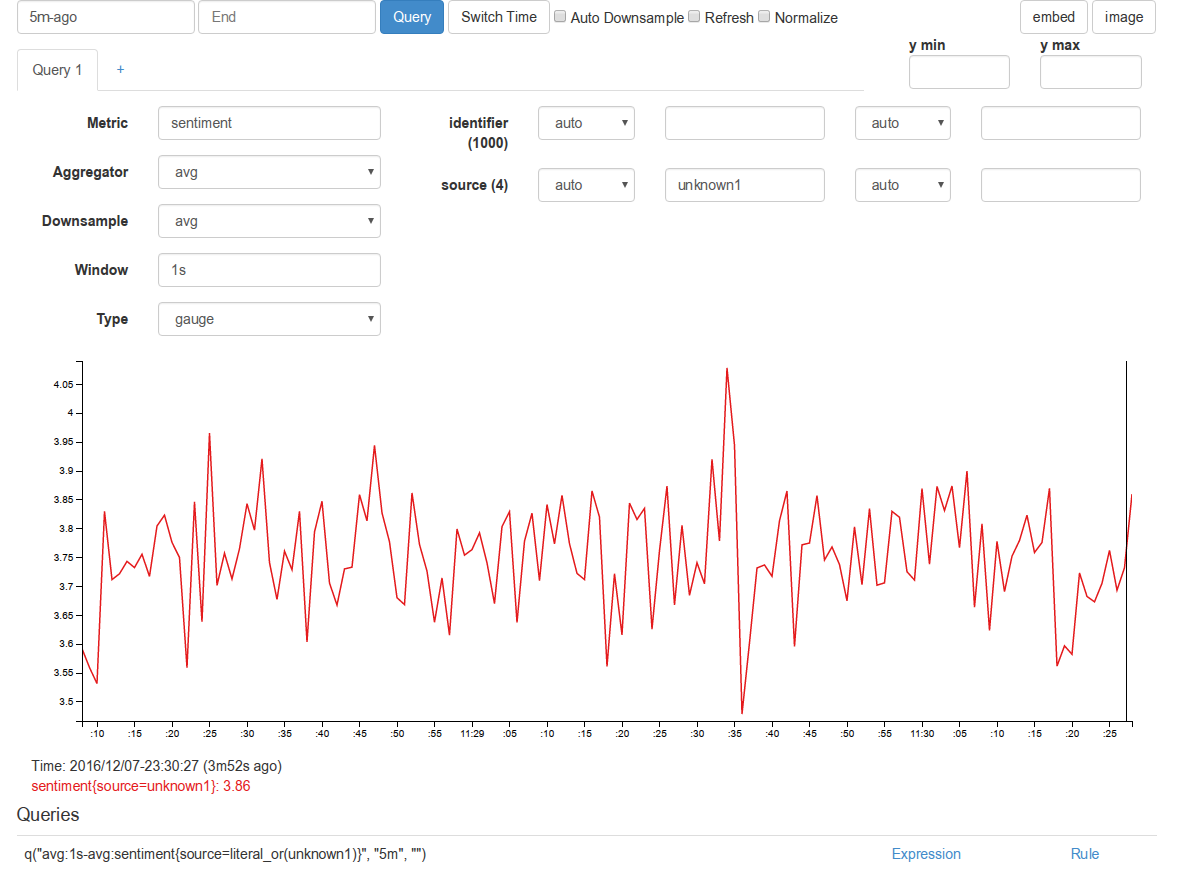
\includegraphics[width=0.9\textwidth]{images/bosun_dash_1.png}
    \caption{Time Series Analytics Dashboard}
\end{figure*}

\begin{figure*}[ht] \label{fig:accuracy-v-data}
    \centering
    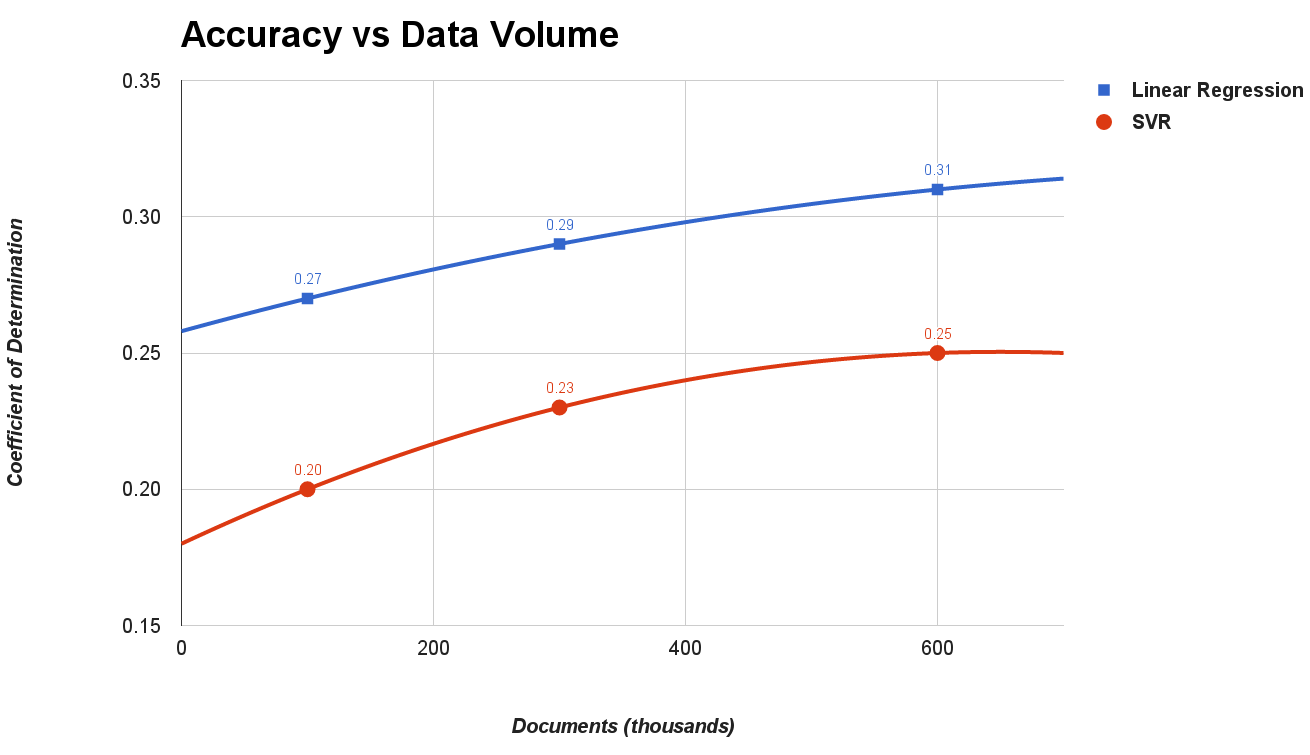
\includegraphics[width=\textwidth]{images/accuracy-vs-data.png}
    \caption{Accuracy vs. Data}
\end{figure*}

\vspace{5mm}

\section{Evaluation}

    \subsection{Testbed}
        The testbed is integrated into the actual framework, and the processors for model training.
        The tests were carried out on an Amazon document corpus of 600,000 unique product reviews.
        The complete dataset of Amazon reviews is openly accessible\cite{amazon_datasets}.

    \subsection{Metrics}
        The experimental results are being evaluated for goodness of model fit using the co-efficient of determination metric \cite{jaeger1990statistics}.
        The co-efficient of determination conveys the quantized amount of signal of the input vector that is being captured by the trained model by validating it against a test set. 
        The value of the co-efficient of determination is derived from the below equations:

        \begin{equation}
            \displaystyle SS_{tot} = \sum_{i} (y_i - \hat{y})^2
        \end{equation}

        \begin{equation}
            \displaystyle SS_{res} = \sum_{i} (f(x)_i - \hat{y})^2
        \end{equation}

        \begin{equation} \label{eq:r_squared}
            \displaystyle R^2 = 1 - \frac{SS_{res}}{SS_{tot}}
        \end{equation}

        The $R^2$ score derived in Equation \ref{eq:r_squared} is the the co-efficient of determination use to predict the goodness of fit for each of the machine learning models learnt.


    \subsection{Experimental Results}
        The accuracy schores of the experimental results are presented in Table \ref{results}. The score presented in this table is the co-efficient of determination or $R^2$ score.

        \begin{table}[ht] \caption{Evaluation results} \label{results}
            \centering
            \resizebox{0.35\textwidth}{!}{
                \begin{tabular}{| c | c |}
                    \hline
                    \textbf{Modeling Method} & \textbf{Score} \\
                    \hline
                    Linear Regression & 0.31 \\
                    \hline
                    Support Vector Regression & 0.25 \\
                    \hline
                \end{tabular}
            }
        \end{table}

        The positive scores of both the experiment analyses indicate that the model does capture a good amount of the sentiment in each of the labeled documents, and ensures a reasonable amount of accuracy for the prediction of the real-time unlabeled documents.

        As indicated in Figure \ref{fig:accuracy-v-data}, the current trend seems to suggest a polynomial improvement on increasing the number of documents to be trained on. 
        The initial experimentation was done on a corpus of 100,000 labeled documents. 

        Also, from the code profiling information presenting in Figure \ref{fig:code-profiling}, it is evident that the unsupervised learning segement of obtaining the document vectors of the labeled documents is the longest running part of the Offline learning module. In comparison, the document processing and statistical model training is negligible.

\begin{figure*}[ht]
    \centering
    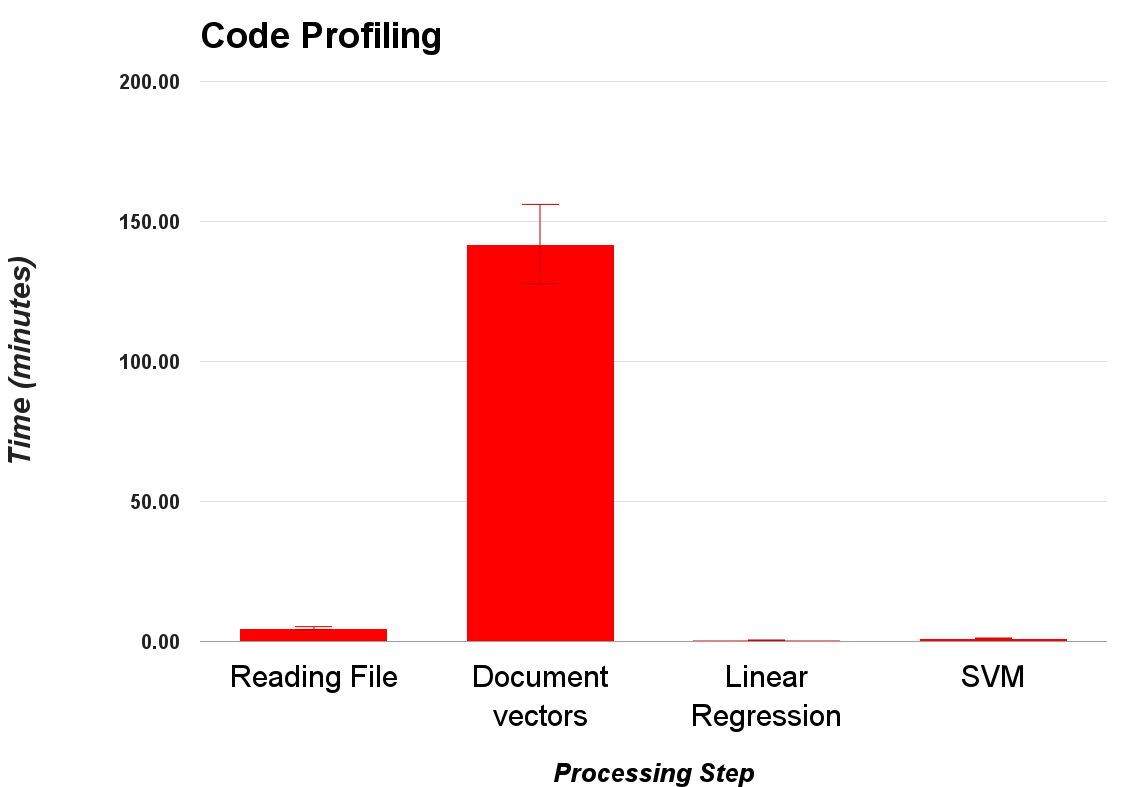
\includegraphics[width=0.8\textwidth]{images/code_profiling.png}
    \caption{Code Profiling Statistics}
    \label{fig:code-profiling}
\end{figure*}

\vspace{5mm}

\section{Conclusions}
    To summarize, this research project encapsulated the below objectives:
    \begin{itemize}
        \item Evaluating the usage of document embeddings for a regression task
        \item Building a framework to predict real-time sentiment trends
    \end{itemize}

    Given that the attempt is to infer sentiment from unstructured data, the result of having a positive $R^2$ value is promising (Table \ref{results}).
    It indicates that the model captures a significant amount of the signal present in the independent variable.
    It can hence be relied to a degree of confidence to predict a close enough value to the actual intended document sentiment.

    Additionally, this work has resulted in a generic framework that can be adopted to build a sentiment analytics dashboard on a user friendly interface. 
    This framework can be extended to processes any type of document content both for training and for the real-time sentiment prediction module.

    The overall framework has been built using state-of-the-art product offering in neural-net document embedding libraries, distributed stream processing in Spark, distributed queue architecture in Kafka, and the stable machine learning framework which is a part of scikit-learn. 

    The author believes this framework can be used both in industrial settings as well as an evaluation testbed for any document embedding and machine learning libraries used as an ensemble. The hypothesis made prior to undertaking this research project, as described in the Problem Statement (Section \ref{problem_statment}) has been validated and proved to be true.

\vspace{5mm}

\section{Future Work}
    With respect to the statistical models trained, the current approach supports only the simplest regression models i.e. Linear Regression and Support Vector Regression (SVR). 
    This could be expanded to offer additional training mechanisms that can integrate more sophisticated regression algorithms for a higher level of accuracy.
     
    Additional channels could be chosen as the culminiation point of the newly rated unlabeled documents.
    For now, the data is stored in a time-series database.
    But this can easily be converted into something more generic, like publishing it to another Kafka queue.
    Mulitple consumer applications can, thus, benefit from the stream of insights published to the stream.

    Another potential aim for future work is to reduce the time taken for the initial document vector training of the offline model.
    As shown in the code profiling statistics present in Figure \ref{fig:code-profiling}, it is evident that a significant redu
    ction in the cost of training the initial model could be acheived if the document vectors training time were to be reduced.

\vspace{5mm}

\section{Acknowledgments}
    The author would like to thank Dr. Paulo Alencar, for his guidance, feedback and suggestions during the conceptualization of this research project.

\vspace{5mm}

\bibliographystyle{abbrv}
\bibliography{cs846-course-project_vineet}

\end{document}
